\documentclass[tikz,border=2pt]{standalone}
\usepackage{amsmath}
\usetikzlibrary{arrows.meta}
\begin{document}
% Counting process A(t) = max{k : A_k <= t} for arrivals A = (1,2,5,9,10): right-continuous
% staircase (filled dot = value at the jump, open dot = left limit); A(6) = 3 and A_{A(6)} = A_3 = 5.
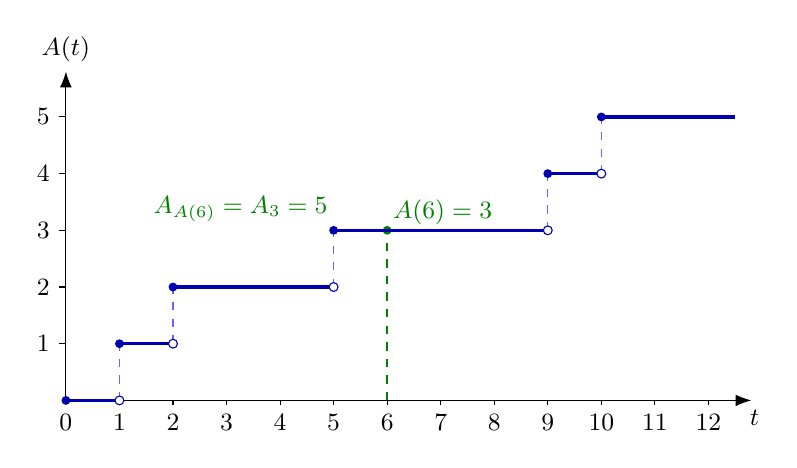
\begin{tikzpicture}[font=\small, >={Latex[length=2mm]}, x=0.68cm, y=0.72cm]
  \draw[->] (0,0) -- (12.8,0) node[anchor=north west, xshift=-4pt] {$t$};
  \draw[->] (0,0) -- (0,5.8) node[anchor=south] {$A(t)$};
  \foreach \t in {0,1,...,12} \draw (\t,0) -- (\t,-0.08) node[below] {$\t$};
  \foreach \n in {1,...,5} \draw (0,\n) -- (-0.12,\n) node[left] {$\n$};
  % guide at t = 6
  \draw[green!50!black, thick, dashed] (6,0) -- (6,3);
  \fill[green!50!black] (6,3) circle (1.6pt);
  \node[green!50!black, anchor=south west, inner sep=2pt] at (6,3) {$A(6)=3$};
  \node[green!50!black, anchor=south east, inner sep=2pt] at (5,3.05) {$A_{A(6)}=A_3=5$};
  % staircase: flat pieces, risers dashed
  \foreach \a/\b/\n in {0/1/0, 1/2/1, 2/5/2, 5/9/3, 9/10/4, 10/12.5/5}
    \draw[blue!70!black, very thick] (\a,\n) -- (\b,\n);
  \foreach \a/\n in {1/1, 2/2, 5/3, 9/4, 10/5} {
    \draw[blue!60, thin, dashed] (\a,\n-1) -- (\a,\n);
    \draw[blue!70!black, fill=white] (\a,\n-1) circle (1.6pt);
    \fill[blue!70!black] (\a,\n) circle (1.6pt);
  }
  \fill[blue!70!black] (0,0) circle (1.6pt);
\end{tikzpicture}
\end{document}
